\section{Fundamentals of Neural Networks}
\label{sec:nn}

Artificial neural networks (NN) are based on the idea of simulating 
the functioning of neuron connections of the human brain. 
%
This machine learning technique is trained in a fashion similar to 
human learning with the goal to process complex inputs and conclude correct outputs \cite{greplova}.
%
A neural network is defined by a (usually large) number of neurons 
interconnected with strength parameters called weights. 

\begin{figure}[H]
    \centering
    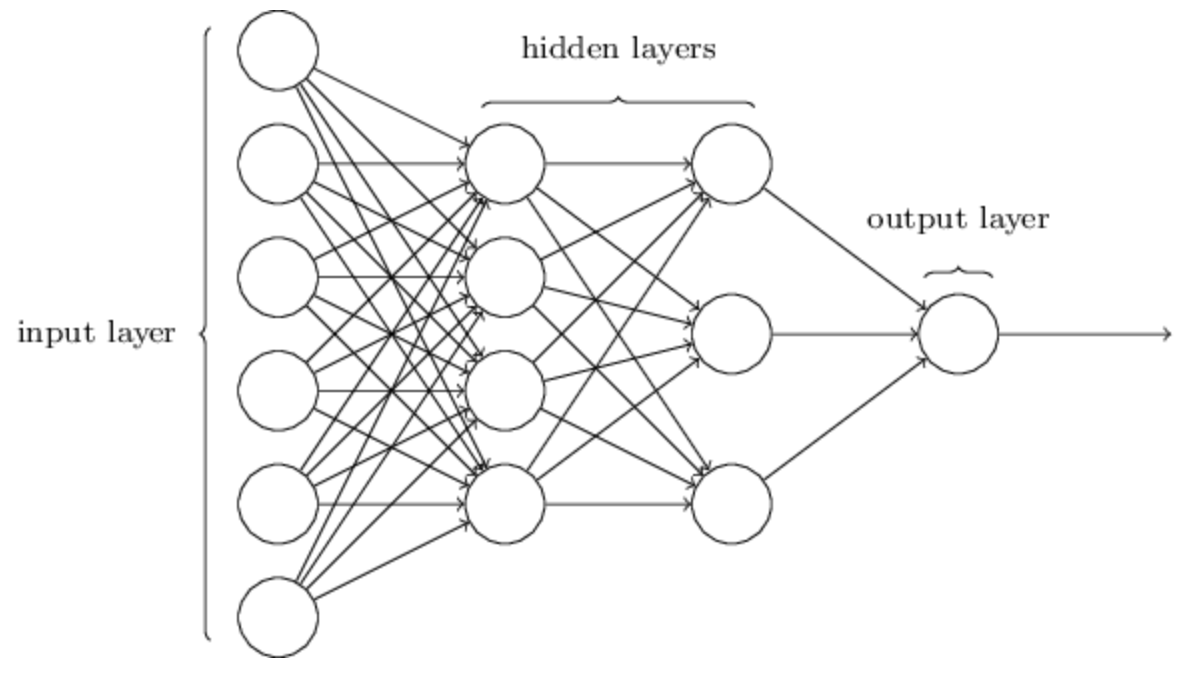
\includegraphics[width=100mm]{plots/nn.png}
    \caption{Schematic representation of a four-layer Neural Network with two hidden layers and one output neuron}
    \label{fig:nn}
\end{figure}

%
Each neuron, represented in the above figure with a circle, 
is connected to a number of neurons in the previous layer and 
its output is the result of an activation function to its inputs:

\begin{equation}
    z = \sum_j w_j x_j + b,
\end{equation}

where $x_j$ are the outputs of the preceding neurons, 
$w_j$ are the corresponding weights and $b$ is the bias (offset) of the neuron. 
%
It is the latter two that will be optimized by training.
A nonlinear activation function $f(z)$ is applied to come to the output value for each neuron; 
this procedure is called forward propagation. 
%
Typical examples for $f(z)$ are the Rectified Linear Unit (ReLU) 
and sigmoid function, as depicted in Fig. \ref{activation}. 
%
Note that these are two often-used, but not the only possible activation functions. 
%
The choice of non-linear activation function influences computational and 
training properties of the neural nets \cite{juan}.
%
For example, choice for the ReLU function ensures absolute positivity. 

\begin{figure}[H]
    \centering
    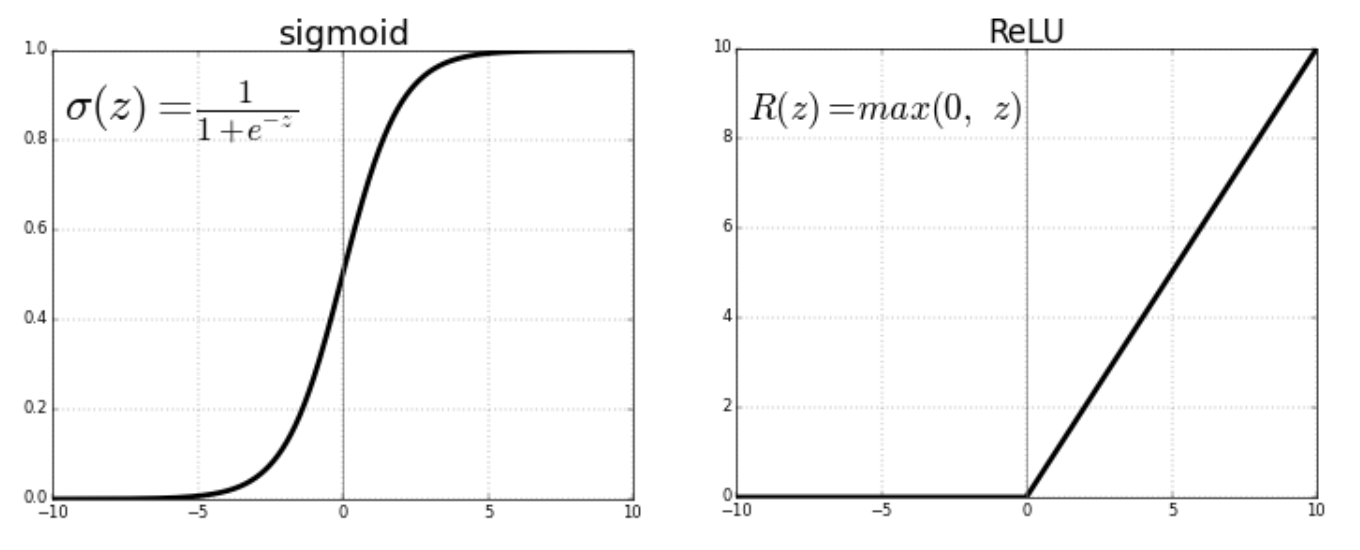
\includegraphics[width=100mm]{plots/f(z).png}
    \caption{Sigmoid (left) and ReLU (right) activation functions. Both approach 0 as $z\rightarrow -\infty$ but note the different behaviour for $z\gg0$. }
    \label{activation}
\end{figure}


For a certain set of inputs \textbf{$x_0$} and a collection of weights and biases $(w^l_j,b^l_j)$, 
with $w^l_j$ being the j-th neuron in the l-th layer.
%
The neural network gives an output $y$ that can be compared to the desired output $y_{target}$. 
%
A cost function $C(y, y_{target})$ is used to quantify how 'far' we are from our desired output, 
and training the algorithm is done by minimizing the cost function with respect to all $(w^l_j,b^l_j)$ of the system. 
%
This minimization is done by means of the gradient descent method, which means 
that after each iteration the weights and biases are adjusted a bit towards 
the minimum of the cost function. 
%
To make this minimization computationally tractable, 
the so-called back-propagation algorithm is being used \cite{hn}, 
allowing us to approximate the derivative of the cost function by averaging over the training set. 
%
All together, training the network relies on the following four fundamental equations:

\begin{align}
\label{eqs3}
\begin{split}
 \delta_j^L &= \frac{\partial C}{\partial a_j^L} f'(z_j^L), 
 \\
 \delta^l &= (w^{l+1} \delta^{l+1}) \odot f'(z^l),
 \\
 \frac{\partial C}{\partial b_j^l} &= \delta_j^l,
 \\
 \frac{\partial C}{\partial w_{jk}^l} &= a_k^{l-1}\delta_j^l.
\end{split}
\end{align}

Here, $\delta_j^l$ is the error and $a_j^l$ the output of neuron $j$ in layer $l$, 
$C$ is the cost, $b$ is the bias and $w$ is the weight of each neuron. 
%
It is the error $\delta_j^L$ that represents the total cost of the network.
%
The last two equations evaluate the gradient of the model parameters 
with the gradient of the cost function. 
%
With this info one can update the model parameters by

\begin{align}
\begin{split}
 b^{l+1} &= b^l - \eta \frac{\partial C}{\partial b^l}
 \\
 w^{l+1} &= w^l - \eta \frac{\partial C}{\partial w^l}
\end{split}
\end{align}
where $\eta$ is the pre-defined learning rate, a measure for the size 
of the step taken with each iteration.
From equations (\ref{eqs3}), one can see that the choice of non-linear 
activation function ($f(z)$) influences the learning of the network. 
%
This can already be deduced from the shape of the functions in Fig.~\ref{activation}: 
since $\sigma$(z) saturates for large inputs $z\gg0$, 
$d\sigma/dz\rightarrow0$ and the network loses sensitivity~\cite{juan}.



We use the definition {\it epoch} for each time that
the entire set of training data is passed forward once through the neural network 
and the network has backpropagated the error and updated all of its parameters
accordingly. 
%
The network needs much more than just one epoch to optimize by means of 
gradient descent, as this is an iterative process. 
%
After each epoch, the performance of the network is evaluated by calculating
the error ($ \delta_j^L$) on the training data and the weights and biases
are adjusted accordingly.
%
As the number of epochs increases, the network parameters are adjusted
repeatedly and where the network was first underfitting the inputs at
the beginning, at a certain moment it goes to optimal fitting,
before it enters the overfitting regime.
%
Several methods can be applied to determine the optimal stopping point
of the network, that is, to find the moment at which the network is
neither under-, nor overfitting the training data. 
%
One of such is splitting the total set of experimental data into two sets:
the training dataset is the one we use to train the model, usually
80\% of the total set.
%
The other 20\% is what we call the validation set and it is used to provide
an unbiased evaluation of the model fit on the training set. 
%
This split ratio is common for models with a moderate number of hyperparameters:
increasing the size or increasing the tunability of the model usually goes with increasing the share of the
validation set. 
%
The validation subset is left out of the training set on purpose and the model
can not learn on this data points.
%
After each epoch, the total performance of the
system can be validated by feeding this subset to the network and calculating
the total error on this data.
%
Tracing the cost function on both the training and the validation set 
gives insight in if the network is overfitting the training data.
First, both the training and validation error will be decreasing, 
but at a certain point the network will start overfitting and the
validation error slowly starts to increase. 
%
The optimal stopping point is defined as the global minimum of the 
error of the validation sample, computed over a large fixed number of 
iterations.
%
A typical progress of the training and validation error over the 
course of the optimization can be observed in Fig.~\ref{fig:cost}.

\begin{figure}[H]
    \label{fig:costs}
    \centering
    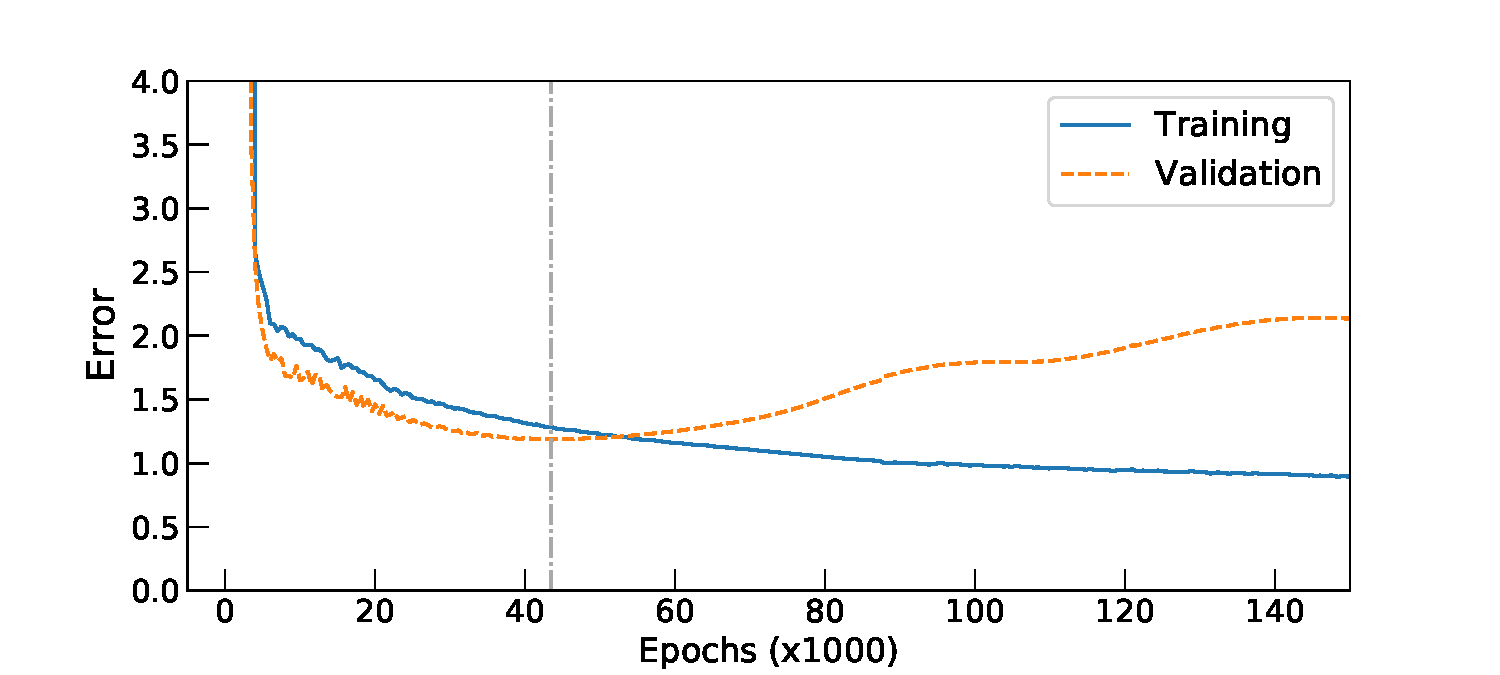
\includegraphics[width=120mm]{plots/train_val_error.pdf}
    \caption{Progress of both the training and validation error over 
    one training session as a function of the number of epochs. 
The optimal stopping point is where the validation error is at
its absolute minimum, here after 43,500 epochs.}

\end{figure}

%
Once the optimal network parameters have been determined and stored, 
the network can be used to
make predictions on any set of inputs. 






